\documentclass{beamer}

\usepackage[utf8]{inputenc}
\usepackage[T1]{fontenc}
\usepackage{amsmath}
\usepackage{amssymb}
\usepackage{amsthm}
\usepackage{graphicx}
\usepackage{hyperref}
\usepackage{booktabs}
\usepackage{bm}
\usepackage{enumerate}
\usepackage{tikz}
\usepackage{tikz-3dplot}
\usetikzlibrary{math}

% Mathematical commands
\newcommand{\E}{\mathbb{E}}
\newcommand{\R}{\mathbb{R}}
\newcommand{\N}{\mathbb{N}}
\newcommand{\C}{\mathbb{C}}
\newcommand{\I}{\mathbf{I}}
\newcommand{\NN}{\mathcal{N}}
\newcommand{\norm}[1]{\left\lVert#1\right\rVert}
\newcommand{\abs}[1]{\left\lvert#1\right\rvert}
\newcommand{\evmin}[1]{\lambda_{\min}\left(#1\right)}
\newcommand{\evmax}[1]{\lambda_{\max}\left(#1\right)}
\newcommand{\svmin}[1]{\sigma_{\min}\left(#1\right)}
\newcommand{\tr}{\text{tr}}
\newcommand{\KNTK}{K_{\text{NTK}}}
\newcommand{\Kinf}{K^{\infty}}
\newcommand{\Sd}{\mathbb{S}^{d-1}}
\newcommand{\Lap}{\Delta}
\newcommand{\Ls}{\mathcal{L}_s}
\newcommand{\limiting}[1]{#1^{\infty}}

\usetheme{Madrid}
\usecolortheme{default}

\title{Spectral Analysis of the Neural Tangent Kernel}
\subtitle{And its Modification by Sobolev-type Training}
\author{Synthesis and Analysis}
\date{\today}

\begin{document}

\begin{frame}
\titlepage
\end{frame}

\begin{frame}{Outline}
\tableofcontents
\end{frame}

\begin{frame}{Eigenvalue Scaling Laws and Learning}
\textbf{Key objectives:}
\begin{itemize}
\item Obtain eigenvalue scaling laws with respect to decay rate: $\mu_\ell \sim \ell^{-\alpha}$
\item Understand spectral properties' impact on learning dynamics
\item Derive scaling laws for eigenvalues w.r.t. network depth $l$ and data size $n$
\end{itemize}

\textbf{NTK Matrix Spectrum approximates Operator Spectrum:}
\begin{itemize}
\item Discrete NTK matrix eigenvalues $\approx$ continuous NTK operator eigenvalues
\item Matrix spectral analysis reveals learning behavior
\end{itemize}

\textbf{Scaling with depth $l$ and data size $n$ (from mlps\_at\_eoc\_1.tex):}
\begin{itemize}
\item Condition number: $\kappa(K^{\infty}) \sim 1 + \frac{n}{3} + \mathcal{O}(n \xi / l)$
\item Eigenvalues: $\lambda \sim \frac{l}{4} \pm \xi$ where $\xi \sim \log(l)$
\item Parameter dependence: scaling controlled by $\Delta_\phi = \frac{b^2}{a^2+b^2} = 0.5$ (ReLU)
\item Results available for all Leaky ReLU activations
\end{itemize}

\textbf{Learning implications:} Eigenvalue decay determines which frequencies are learned fastest
\end{frame}

\section{Sobolev Spaces on Spheres}

\begin{frame}{Distribution Space and Sobolev Operator}
\begin{itemize}
\item Let $\mathcal{D}'(\Sd)$ be the space of distributions on $\Sd$
\item For $s \in \R$, define operator $\Ls: \mathcal{D}'(\Sd) \to \mathcal{D}'(\Sd)$:
\[ \Ls = \I + (-\Lap)^{1/2s} \]
where $\Lap$ is the Laplace-Beltrami operator
\end{itemize}
\end{frame}

\begin{frame}{Spherical Sobolev Spaces}
\begin{itemize}
\item Define $H^s(\Sd) = \{f \in \mathcal{D}'(\Sd) : \Ls f \in L^2(\Sd)\}$
\item Equipped with norm:
\[ \|f\|^2_{H^s(\Sd)} = \sum_{\ell=0}^{\infty} \sum_{p=1}^{N(d,\ell)} (1+\ell)^{2s} |\hat{f}_{\ell,p}|^2 \]
where $\hat{f}_{\ell,p}$ are spherical harmonic coefficients
\end{itemize}
\end{frame}

\begin{frame}{Modified Loss Function}
\begin{itemize}
\item Replace standard $L^2$ loss with Sobolev loss:
\[ \frac{1}{2}\|g-N\|^2_{H^s} \text{ instead of } \frac{1}{2}\|g-N\|^2_{L^2} \]
\item Effects of $s$ parameter:
\begin{itemize}
\item $s = 0$: Reduces to $L^2$ norm
\item $s > 0$: Amplifies high-frequency components by $(1+\ell)^{2s}$
\item $s < 0$: Dampens high-frequency components, more robust to noise
\end{itemize}
\end{itemize}
\end{frame}

\begin{frame}{Regularity Results}
\begin{theorem}[ReLU Network Regularity]
For a 2-layer ReLU network $N: \Sd \to \R$:
\begin{itemize}
\item $N \in H^s(\Sd)$ for all $s < 3/2$
\item For $s \geq 3/2$, $N \in H^s(\Sd)$ if and only if $N$ is affine
\end{itemize}
\end{theorem}
\end{frame}

\begin{frame}{Discretized Sobolev Loss}
\begin{equation*}
\Phi_s(W) = \frac{1}{2} \sum_{\ell=0}^{\ell_{\max}} \sum_{p=1}^{N(d,\ell)} (1+\ell)^{2s} \left|\sum_{i=1}^n c_i Y_{\ell,p}(x_i)(g-N)(x_i)\right|^2
\end{equation*}
\begin{itemize}
\item Equivalent matrix form:
\[ \Phi_s(W) = \frac{1}{2}(y-u)^\top P_s(y-u) \]
where $P_s = \sum_{\ell=0}^{\ell_{\max}} \sum_{p=1}^{N(d,\ell)} (1+\ell)^{2s}P_{\ell,p}$
\item Plus précisément:
\[ P_s = \sum_{\ell=0}^{\ell_{\max}} \sum_{p=1}^{N(d,\ell)} (1+\ell)^{2s}P_{\ell,p}, \quad P_{\ell,p} = a_{\ell,p}a_{\ell,p}^\top, \quad (a_{\ell,p})_i = c_iY_{\ell,p}(x_i) \]
\end{itemize}
\end{frame}

\begin{frame}{What's P}
\begin{itemize}
\item [Placeholder: Definition and properties of operator P]
\item [Placeholder: Mathematical formulation]
\item [Placeholder: Role in Sobolev training]
\item [Placeholder: Connection to spherical harmonics]
\end{itemize}
\end{frame}

\begin{frame}{Chebyshev Nodes or Uniform Nodes, FFT, Tensor in d dim}
\begin{itemize}
\item [Placeholder: Comparison of node distributions]
\item [Placeholder: Fast Fourier Transform implementation]
\item [Placeholder: Tensor product structures in d dimensions]
\item [Placeholder: Computational complexity analysis]
\item [Placeholder: Numerical stability considerations]
\end{itemize}
\end{frame}

\begin{frame}{The Operator Form}
\begin{itemize}
\item Kernel integral operators in $\R^d$:
\[ (\mathcal{K} f)(x) = \int_{\R^d} K(x, x') f(x') dx' \]
\item Kernel integral operators on the sphere $\Sd$:
\[ (\mathcal{K} f)(x) = \int_{\Sd} K(x, x') f(x') d\sigma(x') \]
\item Sobolev operator $P_s$ as integral operator:
\[ (P_s f)(x) = \int_{\Sd} P_s(x, x') f(x') d\sigma(x') \]
\item [Placeholder: Spectral properties comparison]
\item [Placeholder: Eigenfunction analysis]
\end{itemize}
\end{frame}

\begin{frame}{From Sobolev Loss to Fourier Space Operator}
\textbf{Sobolev loss with gradients:}
\[ \mathcal{L}_s[f] = \|f\|_{L^2}^2 + \|\nabla f\|_{L^2}^2 = \int_{\Sd} f(x)^2 d\sigma(x) + \int_{\Sd} \|\nabla f(x)\|^2 d\sigma(x) \]

\textbf{Fourier decomposition:} $f(x) = \sum_{\ell,p} \hat{f}_{\ell,p} Y_{\ell,p}(x)$
\[ \mathcal{L}_s[f] = \sum_{\ell=0}^{\infty} \sum_{p=1}^{N(d,\ell)} (1+\ell)^{2s} |\hat{f}_{\ell,p}|^2 \]

\textbf{Discretization at points $\{x_i\}_{i=1}^n$:}
\[ \hat{f}_{\ell,p} \approx \sum_{i=1}^n c_i f(x_i) Y_{\ell,p}(x_i) \]

\textbf{Matrix form:} $P_s = \sum_{\ell,p} (1+\ell)^{2s} a_{\ell,p} a_{\ell,p}^T$
where $(a_{\ell,p})_i = c_i Y_{\ell,p}(x_i)$

\textbf{Final form:} $\mathcal{L}_s[f] \approx f^T P_s f$ with $f = (f(x_1), \ldots, f(x_n))^T$
\end{frame}

\begin{frame}{Generalization to Any Distribution}
\textbf{Commutation for any distribution $\rho$:}
\begin{itemize}
\item Operators $K$ and $P_s$ commute: $[K, P_s] = 0$
\item This holds for any sampling distribution $\rho(x)$ on $\Sd$
\end{itemize}

\textbf{Quadrature weights and inverse distribution:}
\[ c_i = \frac{1}{\rho(x_i)} \quad \text{(inverse of distribution)} \]

\textbf{Induced scalar product:}
\[ \langle f, g \rangle_\rho = \int_{\Sd} f(x) g(x) \rho(x) d\sigma(x) \approx \sum_{i=1}^n f(x_i) g(x_i) c_i \]

\textbf{Orthogonal eigenvectors:}
\begin{itemize}
\item Spherical harmonics $Y_{\ell,p}$ remain eigenfunctions
\item Orthogonal w.r.t. $\langle \cdot, \cdot \rangle_\rho$: $\langle Y_{\ell,p}, Y_{\ell',p'} \rangle_\rho = \delta_{\ell,\ell'} \delta_{p,p'}$
\item Results extend to any distribution via this weighted inner product
\end{itemize}
\end{frame}

\begin{frame}{Counting Spherical Harmonics}
\textbf{Number of spherical harmonics of degree $\ell$ on $\Sd$:}
\[ N(d,\ell) = \binom{2\ell + d - 2}{d - 2} \]

\textbf{Special cases:}
\begin{itemize}
\item $d = 2$ (circle $\mathbb{S}^1$): $N(2,\ell) = \begin{cases} 1 & \text{if } \ell = 0 \\ 2 & \text{if } \ell \geq 1 \end{cases}$
\item $d = 3$ (sphere $\mathbb{S}^2$): $N(3,\ell) = 2\ell + 1$
\item $d = 4$ (3-sphere $\mathbb{S}^3$): $N(4,\ell) = (\ell + 1)^2$
\end{itemize}

\textbf{Total number up to degree $L$:}
\[ \sum_{\ell=0}^{L} N(d,\ell) = \binom{L + d}{d} \]

\textbf{Asymptotic growth:}
\[ N(d,\ell) \sim \frac{2\ell^{d-2}}{(d-2)!} \quad \text{as } \ell \to \infty \]
\end{frame}

\section{Empirical Results}

\begin{frame}{Theoretical Background: NTK at Edge of Chaos}
\begin{itemize}
\item For MLPs with $(a,b)$-ReLU: $\phi(s) = as + b|s|$
\item At Edge of Chaos (EOC): $\sigma^2 = (a^2+b^2)^{-1}$
\item Key parameter: $\Delta_\phi = \frac{b^2}{a^2+b^2}$
\item Cosine map $\varrho(\rho)$:
\[ \varrho(\rho) = \rho + \Delta_\phi \frac{2}{\pi}\left( \sqrt{1-\rho^2} - \rho \arccos(\rho) \right) \]
\end{itemize}
\end{frame}

\begin{frame}{Limiting NTK Properties}
\begin{itemize}
\item Limiting NTK at EOC:
\[ K^{\infty}(\mathbf{x}_1, \mathbf{x}_2) = \|\mathbf{x}_1\| \|\mathbf{x}_2\| \left( \sum_{k=1}^l \varrho^{\circ (k-1)}\left(\rho_1^{\infty}(\mathbf{x}_1, \mathbf{x}_2)\right) \prod_{k'=k}^{l-1} \varrho'\left(\varrho^{\circ (k'-1)}\left(\rho_1^{\infty}(\mathbf{x}_1, \mathbf{x}_2)\right)\right) \right) \mathbf{I}_{m_l} \]
\item Integral operator:
\[ (\mathcal{L} z)(\mathbf{x}) = \int_{\mathbb{S}^{d-1}} K^{\infty}(\mathbf{x}, \mathbf{x}') z(\mathbf{x}') d\mathbf{x}' \]
\item Eigenvalues decay: $\mu_\ell = \mathcal{O}(\ell^{-d})$
\item \textbf{Deep NTK decay:} For $L$-layer ReLU network with $L \geq 3$:
\[ \mu_k \sim C(d, L)k^{-d} \]
where $C(d, L)$ depends on parity of $k$ and grows quadratically with $L$
\item For normalized NTK $\kappa^L_{\text{NTK}}/L$: $C(d, L)$ grows linearly with $L$
\end{itemize}
\end{frame}

\begin{frame}{Spectral Analysis with Sobolev Training}
\begin{itemize}
\item Final spectral exponent: $2s-d$
\item Cases:
\begin{itemize}
\item $s = d/2$: Balanced learning (flat spectrum)
\item $s > d/2$: High frequencies amplified
\item $s < d/2$: Low frequencies still favored
\end{itemize}
\item Effective eigenvalues:
\[ \lambda_\ell(K_S) = \lambda_\ell(\mathcal{L}) \cdot \lambda_\ell(P_s) \sim \ell^{-d} \cdot \ell^{2s} = \ell^{2s-d} \]
\end{itemize}
\end{frame}

\begin{frame}{Common Eigenfunctions Property}
\begin{theorem}[Spherical Harmonics as Common Eigenfunctions]
For rotationally invariant kernels on $\mathbb{S}^{d-1}$:
\begin{itemize}
\item NTK operator $\mathcal{L}$ and Sobolev operator $P_s$ share spherical harmonics $Y_{\ell,p}$ as eigenfunctions
\item Due to rotational invariance and Schur's lemma
\item Enables direct spectral modification analysis
\end{itemize}
\end{theorem}
\end{frame}

\begin{frame}{Commutation with Laplace-Beltrami}
\begin{theorem}[Commutation Property]
The NTK operator $\mathcal{L}$ and Sobolev operator $P_s$ commute with the Laplace-Beltrami operator $\Lap$:
\[ \Lap \mathcal{L} = \mathcal{L} \Lap \quad \text{and} \quad \Lap P_s = P_s \Lap \]
\begin{itemize}
\item Due to rotational invariance
\item Consequence of sharing spherical harmonics as eigenfunctions
\item Implies spectral decompositions are compatible
\end{itemize}
\end{theorem}
\end{frame}

\begin{frame}{Matrix Visualization of Operators}
\begin{columns}
\column{0.33\textwidth}
[Placeholder: Heatmap of NTK matrix $K$]
\column{0.33\textwidth}
[Placeholder: Heatmap of Sobolev matrix $P_s$]
\column{0.33\textwidth}
[Placeholder: Heatmap of combined operator $KP_s$]
\end{columns}
\begin{itemize}
\item Structure of kernel matrices
\item Block-diagonal patterns from spherical harmonics
\item Symmetry properties visible in structure
\end{itemize}
\end{frame}

\begin{frame}{Spectral Analysis}
\begin{columns}
\column{0.5\textwidth}
[Placeholder: Eigenvalue decay plots]
\begin{itemize}
\item $K$: $\sim \ell^{-d}$
\item $P_s$: $\sim \ell^{2s}$
\item $KP_s$: $\sim \ell^{2s-d}$
\end{itemize}
\column{0.5\textwidth}
[Placeholder: Eigenvector correlation plots]
\begin{itemize}
\item Alignment with spherical harmonics
\item Verification of commutation
\item Numerical accuracy
\end{itemize}
\end{columns}
\end{frame}

\begin{frame}{Experimental Validation}
\begin{columns}
\column{0.33\textwidth}
[Placeholder: Learning curves for different $s$]
\column{0.33\textwidth}
[Placeholder: Frequency component evolution]
\column{0.33\textwidth}
[Placeholder: Error vs frequency plots]
\end{columns}
\begin{itemize}
\item Empirical verification of theoretical predictions
\item Convergence rates match spectral theory
\item Effect of $s$ parameter on learning dynamics
\end{itemize}
\end{frame}

\begin{frame}{Training Dynamics Comparison}
[Placeholder: Loss curves]
\begin{columns}
\column{0.5\textwidth}
L2 Loss:
[Placeholder: L2 training curves]
\column{0.5\textwidth}
Sobolev Loss:
[Placeholder: Sobolev training curves]
\end{columns}
\end{frame}

\begin{frame}{DeepONet Performance}
[Placeholder: DeepONet specific results]
\begin{itemize}
\item Various network widths
\item Different depth configurations
\item Convergence analysis
\end{itemize}
\end{frame}

\begin{frame}{Deep Network Analysis}
[Placeholder: Very deep network results]
\begin{itemize}
\item Impact on spectral properties
\item Training stability
\item Convergence rates
\end{itemize}
\end{frame}

\begin{frame}{NTK Analysis of Deep Narrow Neural Networks}
\textbf{Theorem 1 (Scaled NTK at initialization):}
For $f^L_\theta$ initialized appropriately, as $L \to \infty$:
\[ \tilde{\Theta}^L_0(x, x') \xrightarrow{p} \tilde{\Theta}^\infty(x, x') \]
where
\[ \tilde{\Theta}^\infty(x, x') = (x^T x' + 1 + \E_g[\sigma(g(x))\sigma(g(x'))]) I_{d_{out}} \]
with $g \sim \text{GP}(0, \rho^2 d_{in}^{-1} x^T x' + \beta^2)$ (Gaussian random field)

\textbf{Alternative form:} $\kappa_1(\cos(u) \cdot v)$ where:
\begin{itemize}
\item $v = \frac{1}{1 + \beta^2/\alpha^2}$, $\beta$ = bias variance
\item $\alpha = \frac{\|x\| \|x'\| \rho}{d_{in}}$, $\cos(u)$ = cosine distance between $x, x'$
\end{itemize}

\textbf{Promising direction:} Limited expansion analysis for this specific architecture with infinite layers and special initialization (positive entries assumption)
\end{frame}

\begin{frame}{Perspectives}
\textbf{Research directions for deep narrow networks:}
\begin{itemize}
\item \textbf{Concatenate units:} Combine multiple narrow networks to increase expressivity
\item \textbf{Alternative initializations:} Explore different initialization schemes beyond current setup
\item \textbf{$\beta \to 0$ limit:} Analyze behavior when bias variance vanishes
\[ v = \frac{1}{1 + \beta^2/\alpha^2} \to 1 \text{ as } \beta \to 0 \]
\item \textbf{Complex kernel structures:} Find initializations that yield more intricate kernel forms
\item \textbf{Skip connections:} Investigate ResNet-style connections for this framework
\[ \tilde{\Theta}^\infty_{\text{skip}}(x, x') = \tilde{\Theta}^\infty(x, x') + \text{skip terms} \]
\end{itemize}

\textbf{Goal:} Richer spectral properties and improved learning dynamics
\end{frame}

\begin{frame}{Mean Field Analysis and Experimental Validation}
\textbf{Mean Field Analysis:}
\begin{itemize}
\item Extension of Hayou \& Yang's work on ResNets
\item Showed that "wide and deep limits commute" for ResNets
\item Can be applied to our deep narrow framework
\item Theoretical foundation for understanding scaling behaviors
\end{itemize}

\textbf{Additional stochasticity in initialization:}
\begin{itemize}
\item Random weight initialization schemes
\item Stochastic bias initialization patterns
\item Random architectural choices (layer widths, connections)
\item Noise in initial parameter distributions
\end{itemize}

\textbf{Experimental validation:}
\begin{itemize}
\item Test theoretical predictions on practical tasks
\item Compare different initialization schemes
\item Evaluate impact of architectural modifications
\item Benchmark against standard wide networks
\end{itemize}

\textbf{Research strategy:} Theory-guided experiments to identify what works in practice
\end{frame}

\begin{frame}{Inverse Cosine Distance Matrix and Near-Affine NTK Behavior}
\textbf{Inverse cosine distance matrix $W_k$:}
\[ {W_k}_{i,i} = 0, \quad {W_k}_{i_1,i_2} = \left( \frac{1 - \rho_k(x_{i_1},x_{i_2})}{2} \right)^{-\frac{1}{2}} \text{ for } i_1 \neq i_2 \]

\textbf{Key approximation result (Proposition from mlps\_at\_eoc\_1.tex):}
The NTK entries are approximated by inverse cosine distances:
\[ u_k \approx \Delta_\phi^{-1} \frac{3\pi}{16} \omega^{\circ (k-1)}\left( \left( \frac{1-\rho}{2} \right)^{-\frac{1}{2}} \right) - \frac{1}{8} \]

\textbf{Near-affine behavior:}
\begin{itemize}
\item NTK matrix $\limiting{K} \approx A \cdot W_l + B$ (affine dependence)
\item Spectral bounds transfer from $W_k$ to NTK via this affine relationship
\item Error terms: $O(\Delta_\phi^{-2} k^{-1})$ - decreases with depth
\end{itemize}

\textbf{Practical implication:} Analyzing inverse cosine distance matrices gives direct insight into NTK spectral properties
\end{frame}

\section{Advanced Variants}

\begin{frame}{Alternative Approaches}
\begin{itemize}
\item Chebyshev differentiation method
\item Stochastic Jacobian technique
\begin{itemize}
\item Expectation evaluation
\item Computational advantages
\end{itemize}
\item Future research directions
\end{itemize}
\end{frame}

\begin{frame}{Visualization of Points on $\mathbb{S}^1$}
\begin{center}
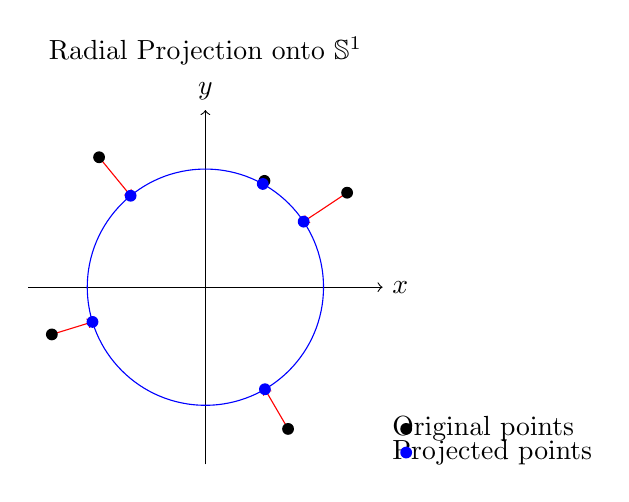
\begin{tikzpicture}[scale=1.5]
    % Draw coordinate axes
    \draw[->] (-1.5,0) -- (1.5,0) node[right] {$x$};
    \draw[->] (0,-1.5) -- (0,1.5) node[above] {$y$};
    
    % Draw the unit circle
    \draw[blue] (0,0) circle (1);
    
    % Draw 10 points with their projections
    % Point 1 (from (1.2, 0.8) to normalized)
    \draw[red,->] (1.2,0.8) -- (0.832,0.555);
    \fill (1.2,0.8) circle (0.05);
    \fill[blue] (0.832,0.555) circle (0.05);
    
    % Point 2 (from (-0.9, 1.1) to normalized)
    \draw[red,->] (-0.9,1.1) -- (-0.633,0.774);
    \fill (-0.9,1.1) circle (0.05);
    \fill[blue] (-0.633,0.774) circle (0.05);
    
    % Point 3 (from (-1.3, -0.4) to normalized)
    \draw[red,->] (-1.3,-0.4) -- (-0.956,-0.294);
    \fill (-1.3,-0.4) circle (0.05);
    \fill[blue] (-0.956,-0.294) circle (0.05);
    
    % Point 4 (from (0.7, -1.2) to normalized)
    \draw[red,->] (0.7,-1.2) -- (0.504,-0.864);
    \fill (0.7,-1.2) circle (0.05);
    \fill[blue] (0.504,-0.864) circle (0.05);
    
    % Point 5 (from (0.5, 0.9) to normalized)
    \draw[red,->] (0.5,0.9) -- (0.486,0.874);
    \fill (0.5,0.9) circle (0.05);
    \fill[blue] (0.486,0.874) circle (0.05);
    
    % Add legend
    \node[right] at (1.5,-1.2) {Original points};
    \fill (1.7,-1.2) circle (0.05);
    \node[right] at (1.5,-1.4) {Projected points};
    \fill[blue] (1.7,-1.4) circle (0.05);
    
    % Add title
    \node[above] at (0,1.8) {Radial Projection onto $\mathbb{S}^1$};
\end{tikzpicture}
\end{center}
\begin{itemize}
\item Points in $\R^2$ projected radially onto $\mathbb{S}^1$
\item Illustrates normalization process
\item Represents sampling from radial distribution
\end{itemize}
\end{frame}

\section{Conclusion}

\begin{frame}{Summary}
\begin{itemize}
\item NTK frequency bias is fundamental
\item Can be tuned via Sobolev training
\item Choice of $s$ parameter controls learning dynamics
\item Opens new perspectives for network training
\end{itemize}
\end{frame}

\end{document}
